\newpage
\section{Échantillonnage statistique}
\begin{figure*}[t]
\centering
\includegraphics[width=0.9\textwidth]{Images/SamplingDesign_\ldoc.png}
\caption{\small Diverses populations et échantillons dans le modèle d'échantillonnage.} \hrule\label{fig:sammod}
\end{figure*}

\begin{tcolorbox}[title=On ne peut pas d\'emontrer le contraire...]
%Figures often beguile me, particularly when I have the arranging of them myself; in which case the remark attributed to Disraeli would often apply with justice and force: 'There are three kinds of lies: lies, damned lies, and statistics.' 
Les derniers sondages suggèrent que 3 personnes sur 4 représentent 75\% de la population globale.\\[-0.6cm]
\begin{flushright}
%-- Mark Twain, \textit{Chapters of My Autobiography}, 1906
-- attribu\'e \`a David Letterman
\end{flushright}
\end{tcolorbox}
\noindent
Bien que le \textit{World Wide Web} contienne des tonnes de données, le grattage du web ne ne permet pas de répondre à la question de la validité des données: les données extraites seront-elles \textbf{utiles} en tant qu'élément analytique? Seront-elles suffisantes pour fournir les réponses quantitatives recherchées? 

Une bonne partie des renseignements qui suivent proviennent de \cite{DC_F,DC_SC}. Une \textbf{enquête} ou un \textbf{sondage} est n'importe quelle activité qui recueille des informations sur des caractéristiques d'intérêt 
\begin{itemize}[noitemsep] 
\item de façon \textbf{organisée} et \textbf{méthodique};
\item couvrant une partie ou la totalité des \textbf{unités} d'une population;
\item utilisant des concepts, méthodes et procédures \textbf{bien définis}, et
\item qui compile ces informations sous une forme récapitulative \textbf{utile}. 
\end{itemize}
Un \textbf{recensement} est une enquête dans laquelle les informations sont recueillies auprès de toutes les unités d'une population, alors qu'une \textbf{enquête par sondage} n'utilise qu'une fraction des unités. 
%\afterpage{\FloatBarrier}
\subsection{Modèle d'échantillonnage}
Lorsque l'échantillonnage est effectué correctement, on peut utiliser diverses méthodes statistiques afin de tirer des conclusions sur la \textbf{population cible} en échantillonnant un nombre (relativement) faible d'unités dans la \textbf{population à l'étude}. La relation entre les différentes populations (\textbf{cible}, à l'\textbf{étude}, \textbf{répondante}) et les échantillons (\textbf{vis\'e}, \textbf{réalisé}) est illustrée à la Figure~\ref{fig:sammod}. 
\subsection{Facteurs déterminants} Dans certains cas, les informations sur la population \textbf{dans son entièreté} sont nécessaires pour répondre à des questions sur la popultion, alors que dans plusieurs cas, elles ne le sont pas.  Comment déterminer quel type d'enquête doit être mené relatif à la collecte des données? La réponse dépend de plusieurs facteurs: 
\begin{itemize}[noitemsep]
    \item le type de question à laquelle il faut répondre;
\item la précision requise;
\item le coût d'étude d'une unité;
\item le temps nécessaire pour enquêter sur une unité;\item  la taille de la population faisant l'objet de l'enquête; et 
\item la prévalence des attributs d'intérêt.
\end{itemize}
Une fois le choix effectué, chaque enquête suit généralement les mêmes \textbf{étapes}:
\begin{enumerate}[noitemsep]
    \item déclaration des objectifs
    \item sélection de la base de sondage
    \item choix d'un plan d'échantillonnage
    \item conception (``design'') du questionnaire
    \item collecte des données
    \item saisie et codage des données
    \item traitement et imputation des données 
    \item estimation 
    \item analyse des données
    \item diffusion et documentation 
\end{enumerate}
Ces étapes ne suivent pas toujours une marche linéaire, dans la mesure où la planification préliminaire et la collecte de données peuvent guider la mise en œuvre (choix d'une base de sondage et d'un plan d'échantillonnage, conception du questionnaire), mais on s'attend à un mouvement général de l'objectif à la diffusion. 
\subsection{Bases de sondage} La \textbf{base de sondage} fournit les moyens d'\textbf{identifier} et de \textbf{contacter} les unités de la population étudiée. En g\'en\'eral, il  peut s'avérer coûteux de la créer et de l'entretenir (en fait, il existe des organisations et des entreprises spécialisées dans la construction et/ou la vente de tels base). Pour être utiles, elles doivent contenir des données:
\begin{itemize}[noitemsep]
\item d'identification des unités;
\item de moyen de contact  des unités;
\item de classification des unités;
\item de mise à jour, et 
\item de couplage de diverses sources.
\end{itemize} La base de sondage idéale doit minimiser le risque de problème avec la \textbf{couverture}, ainsi que le nombre de \textbf{duplications} et de \textbf{misclassifications} (certains de ces problèmes peuvent être r\'esolus au stade du traitement des données).\par À moins que la base de sondage choisie ne soit \textbf{pertinente} (c'est-à-dire qu'elle correspond à la population cible et lui permet d'y accéder), \textbf{précise} (c'est-à-dire que les informations qu'elle contient sont valides),  \textbf{abordable} et \textbf{à jour}, l'approche à base d''échantillonnage statistique est contre-indiquée. 
\subsection{Erreur d'enquête} La capacité à fournir des estimés de diverses quantités d'intérêt dans la population cible, et à permettre le contrôle de l'\textbf{erreur totale} (ET) est l'un des points forts de l'échantillonnage statistique. L'ET d'un estimé est le montant par lequel il diffère de sa valeur réelle dans la population cible:
\begin{align*} 
\text{erreur}&\text{\ totale}  =  \text{erreur\ de\ mesure}  +  \text{erreur\ d'échantillonnage} \\ & +  \text{erreur\ due\ à la non-réponse} +  \text{erreur\ de\ couverture} \\ & + \text{erreur de traitement}, \end{align*}
o\`u 
\begin{itemize}[noitemsep]
\item l'\textbf{erreur de couverture} est due aux différences entre la population à l'étude et à la population cible; 
\item l'\textbf{erreur due \`a la non-r\'eponse} est due aux diff\'erences entre la population r\'epondante et la population \`a l'\'etude;
\item l'\textbf{erreur d'\'echantillonnage} est due aux diff\'erences entre l'\'echantillon r\'ealis\'e et la population r\'epondante; 
\item l'\textbf{erreur de mesure} est due au fait que la valeur réelle de la caract\'eristique d'int\'er\^et n'ayant pas \'et\'e évaluée correctement dans l'\'echantillon r\'ealis\'e, et 
\item l'\textbf{erreur de traitement} est due au fait que la valeur réelle de la caract\'eristique d'int\'er\^et peut \^etre affect\'ee par les transformations de donn\'ees effectu\'ees tout au long de l'analyse. 
\end{itemize}
Soient
\begin{itemize}[noitemsep]
\item $\overline{x}$ la valeur de la caractéristique d'intérêt calculée à l'aide de l'échantillon réalisé; 
\item $\overline{x}_{\mathrm{reel}}$ la valeur r\'eelle de la caractéristique d'intérêt calculée à l'aide de l'échantillon réalisé, en supposant qu'il n'y ait aucune erreur de mesure ou de traitement des donn\'ees; 
\item $x_{\mathrm{rep}}$ la valeur de la caractéristique d'intérêt calculée dans la population r\'epondante;
\item $x_{\mathrm{etude}}$ la valeur de la caractéristique d'intérêt calculée dans la population à l'étude, et 
\item $x_{\mathrm{cible}}$ la valeur de la caractéristique d'intérêt calculée dans la population cible.
\end{itemize}
Alors 
\begin{align*}\text{ET}  &= \overline{x} - x_{\mathrm{cible}}  =  (\overline{x} - \overline{x}_{\mathrm{reel}}) + (\overline{x}_{\mathrm{reel}}-x_{\mathrm{rep}}) \\ &\qquad + (x_{\mathrm{rep}}-x_{\mathrm{etude}}) + (x_{\mathrm{etude}}-x_{\mathrm{cible}}).\end{align*} 
Dans un scénario idéal, $\text{erreur totale}=0$. En réalité, il y a deux contributions principales à l'ET: les \textbf{erreurs d'échan\-til\-lon\-nage} (dont nous parlerons prochainement) et \textbf{les erreurs non dues à l'échantillonnage}, qui comprennent toute contribution à l'erreur d'enquête qui n'est pas due au choix du schéma d'échantillonnage. Cette dernière peut être contrôlée, dans une certaine mesure: 
\begin{itemize}[noitemsep]
\item l'\textbf{erreur de couverture} peut être minimisée en choisissant une base de sondage à jour de haute qualité;
\item l'\textbf{erreur due à la non-réponse} peut être minimisée par un choix judicieux du mode de collecte des données et de la conception du questionnaire, et par l'utilisation de ``rappels'' et de ``suivis'';
\item l'\textbf{erreur de mesure} peut être réduite au minimum par une conception soigneuse du questionnaire, un test préalable de la technique de mesure, et une contre-validation des réponses.  
\end{itemize}
Ces suggestions sont peut-être moins utiles qu'on ne pourrait l'espérer à l'époque moderne: les bases de sondage construites à partir de lignes de téléphone fixes perdent rapidement de leur pertinence compte tenu de la population de plus en plus nombreuse (et jeune) qui évite ce mode de communication, par exemple, tandis que les taux de réponse pour les enquêtes qui ne sont pas obligatoires en vertu de la loi sont étonnamment faibles. Cela explique en partie la tendance vers la collecte automatisée de données et l'utilisation de méthodes d'\textbf{échantillonnage non probabiliste}.     
\subsection{Modes de collecte}
Il existe des approches \textbf{sur papier}, des approches \textbf{assistées par ordinateur} et une série d'autres modes de collecte.
\begin{itemize}
\item Les \textbf{questionnaires auto-administrés} sont u\-ti\-li\-sés lorsque les unités répondantes doivent consulter leurs dossiers personnels afin de fournir les informations demandées (ce qui peut réduire les erreurs de mesure). Ils sont efficaces pour mesurer les réponses aux questions sensibles car ils fournissent une couche supplémentaire de confidentialité. Ils ne sont généralement pas aussi dispendieux que les autres modes de collecte, mais ils ont tendance à être associés à un taux de non-réponse élevé. 
\item Les \textbf{questionnaires assistés par l'enquêteur} u\-ti\-li\-sent des enquêteurs dont la formation permet d'aug\-men\-ter le taux de réponse et la qualité globale des données. Quoique les \textbf{entrevues en personne} permettent d'obtenir des taux de réponse plus élevés, elles sont beaucoup plus dispendieuses, tant au niveau de la formation que des salaires. De plus, il se peut que l'enquêteur doive se rendre à plusieurs reprises chez les répondants sélectionnés avant que le contact ne soit établi. Les \textbf{entrevues téléphoniques}, d'autre part, produisent des taux de réponse ``raisonnables'' à un coût ``raisonnable'' et sont plus sécuritaires pour les intervieweurs, mais leur durée effective est limitée en raison de la ``fatigue t\'el\'ephonique'' des répondants. Pour chaque entretien complété, l'intervieweur passe 4 à 6 minutes en dehors du champ de l'enquête en raison de la composition aléatoire des numéros.
\item Les \textbf{entretiens assistés par ordinateur} combinent la collecte et la saisie des données, ce qui permet de gagner un temps précieux; malheureusement, il y a toujours des unités d'échantillonnage qui n'ont pas accès à un ordinateur/enregistreur de données (bien que cela soit de moins en moins fréquent). Tous les modes papier ont un équivalent assisté par ordinateur: les \textbf{questionnaires auto-administr\'es et assistés par ordinateur}, les \textbf{entretriens assist\'es par ordinateur}, les \textbf{entretiens t\'el\'ephoniques assist\'es par ordinateur}, et les \textbf{interviews en personne assist\'ees par ordinateur}.
\item Les observations directes et discrètes; les carnets de bord à remplir (papier ou électronique); les sondages omnibus, et les questionnaires administr\'e par courriel, sur Internet, et les r\'eseaux sociaux.
\end{itemize}
\subsection{Échantillonnage non probabiliste}
Il y a plusieurs méthodes permettant de choisir des unités d'échantillonnage dans la population cible qui utilisent des approches subjectives et non aléatoires (ENP). Ces méthodes sont souvent \textbf{rapides}, \textbf{relativement peu coûteuses} et \textbf{commodes} dans la mesure où elles ne requierent pas de base de sondage. Les méthodes ENP sont idéales pour l'\textbf{analyse exploratoire} et lors de  l'\textbf{élaboration d'enquêtes}. \par Malheureusement, elles sont parfois utilisées \textbf{au lieu} d'un plan d'échantillonnage probabiliste, ce qui pose des problèmes; le biais de sélection associé rend ces méthodes ENP \textbf{non fiables} relatives aux \textbf{interférences}, car elles ne peuvent être utilisées afin de fournir \textbf{des estim\'es fiables de l'erreur d'échantillonnage}, qui, on le rappelle, est la seule composante de l'erreur totale sur laquelle les analystes ont un contrôle direct. La collecte automatisée de données tombe souvent carrément dans le camp des ENP, par exemple. Bien qu'on puisse toujours analyser les données collectées par une approche ENP, on \textbf{ne peut pas généraliser les résultats} à la population cible (sauf dans des situations rares, de type recensement). \newl
Parmi les m\'ethodes ENP, on compte:
\begin{itemize}[noitemsep]
\item l'échantillonnage \`a l'\textbf{aveuglette}, ou dit de la ``personne de la rue'', consiste \`a choisir les unit\'es comme elle se pr\'esente\`a l'enqu\^eteur; il prend pour acquis que la population est homogène, mais la sélection reste soumise aux biais des enquêteurs et à la disponibilité des unités;
\item l'\'echantillonnage dans lequel les r\'epondants se portent \textbf{volontaire}; il existe un biais de sélection important puisque la majorité silencieuse ne se pr\^ete pas souvent au jeu; cette méthode est souvent imposée aux analystes en raison de considérations éthiques; elle est également utilisée pour les groupes de discussion ou les tests qualitatifs;
\item l'échantillonnage au \textbf{jug\'e} se fonde sur les idées des analystes concernant la composition de la population cible et sur son comportement (au moyen d'une étude préalable, parfois); les unités sont sélectionnées par des experts au sujet de la population, mais des idées préconçues inexactes peuvent introduire des biais importants dans l'étude;
\item L'échantillonnage par \textbf{quotas} est très couramment utilisé (et l'est encore aujourd'hui dans les sondages à la sortie des bureaux de vote en dépit de la  célèbre débâcle ``Dewey Defeats Truman'' de 1948 \cite{DC_DDT}); l'échantillonnage se poursuit jusqu'à ce qu'un nombre spécifique d'unités pour diverses sous-populations ait été sélectionné; il est préférable \`a
 d'autres méthodes ENP en raison de l'inclusion de sous-populations, mais il ignore le biais de non-réponse;
\item L'échantillonnage \textbf{modifié} commence par un échantillonnage probabiliste (nous y reviendrons plus tard), mais passe ensuite à l'échantillonnage de type quota dans, en partie pour faire face à des taux de non-réponse élevés;
\item l'\'echantillonage de type \textbf{boule de neige} demande aux unités échantillonnées de recruter d'autres unités parmi leurs connaissances; cette approche ENP peut aider à localiser des populations cachées, mais elle est biaisée en faveur des unités ayant des cercles sociaux plus larges et des unités qui sont suffisamment charmantes pour convaincre leurs connaissances de participer \`a l'enquête. 
\end{itemize}
Il existe des contextes dans lesquels les méthodes ENP pourraient finir par répondre aux besoins du client (et cela demeure leur décision \`a prendre, au final), mais les analystes DOIVENT tout de même informer le client des inconvénients et leur présenter quelques alternatives probabilistes.  
\subsection{Échantillonnage probabiliste (ou al\'eatoire)}
Les difficult\'es li\'ees aux d\'eductions dans le contexte de l'ENP est une frappe colossale contre leur utilisation. M\^eme si les plans d'échantillonnage probabilistes (ou al\'eatoires) sont généralement \textbf{plus difficiles et plus coûteux} à impl\'ementer (en raison de la nécessité d'une base de sondage de bonne qualité), et prennent \textbf{plus de temps} à réaliser, ils fournissent \textbf{des estim\'es fiables} pour les attributs d'intérêt et pour l'erreur d'échantillonnage, ce qui ouvre la voie à l'utilisation d'échantillons de petite taille afin de tirer des conclusions sur des populations cibles plus vastes (en théorie, du moins; les composantes d'erreur non liées à l'échantillonnage peuvent toujours affecter les résultats et la généralisation). \newl Nous examinerons de plus près des plans d'échantillonnage probabiliste traditionnels tels que l'\'echantillonage \textbf{aléatoire simple}, l'\'echantillonage \textbf{stratifié}, et l'\'echantillonage \textbf{systématique}, -- il existe plusieurs autres variantes: \textbf{par grappes}, avec \textbf{probabilité proportionnelle à la taille},  \`a \textbf{plusieurs degr\'es}, etc.  (consulter \cite{DC_F,DC_SC} pour plus de détails).\newl
Nous commençons par présenter quelques concepts mathématiques fondamentaux. Soit $\mathcal{U}=\{u_1,\ldots,u_N\}$ une population de taille $N<\infty$.  La \textbf{moyenne} et la \textbf{variance} de la population sont respectivement  
$$\mu=\frac{1}{N}\sum_{j=1}^Nu_j\quad\mbox{et}\quad \sigma^2=\frac{1}{N}\sum_{j=1}^N(u_j-\mu)^2.$$ Si $\mathcal{Y}=\{y_1,\ldots,y_n\}$ est un \'echantillon de $\mathcal{U}$, la  \textbf{moyenne empirique} et la \textbf{variance empirique} sont respectivement  
$$\overline{y}=\frac{1}{n}\sum_{i=1}^ny_i\quad\mbox{et}\quad S^2=\frac{1}{n-1}\sum_{i=1}^n(y_i-\overline{y})^2.$$ Soient  $X_1,\ldots,X_n$ des variables al\'eatoires, $b_1,\ldots,b_n\in \mathbb{R}$, et $\GE$, $\GV$, et $\GC$ les op\'erateurs respectifs de l' \textbf{esp\'erance}, de la  \textbf{variance} et de la  \textbf{covariance}. Rappellons que  
\begin{align*}
    \GE \left(\sum_{i=1}^nb_iX_i\right) &=\sum_{i=1}^nb_i\GE(X_i) \\
    \GV\left(\sum_{i=1}^nb_iX_i\right)&=\sum_{i=1}^n b_i^2\GV(X_i)+\sum_{1\leq i\neq j}^nb_ib_j\GC(X_i,X_j) \\
\GC(X_i,X_j)&=\GE(X_iX_j)-\GE(X_i)\GE(X_j)\\
\GV(X_i)&=\GC(X_i,X_i)=\GE\left(X_i^2\right)-\GE^2(X_i).
\end{align*}
L'\textbf{erreur syst\'ematique} (ou biais) d'une composante d'erreur est la moyenne de cette composante lorsque le sondage est répétée \'a maintes reprises (et de façon indépendante) dans les mêmes conditions. La \textbf{variabilité} de cette m\^eme composante d'erreur est la mesure dans laquelle cette composante varie par rapport à sa valeur moyenne dans le scénario idéal décrit ci-dessus. L'\textbf{erreur quadratique moyenne} ($\MSE$) de la composante d'erreur est une mesure de la magnitude de cette erreur:
\begin{align*}
\MSE(\hat{\beta})&=\GE\left((\hat{\beta}-\beta)^2\right)=\GE\left((\hat{\beta}-\GE(\hat{\beta})+\GE(\hat{\beta})-\beta)^2\right)\\&=\GV(\hat{\beta})+\left(\GE(\hat{\beta})-\beta\right)^2=\GV(\hat{\beta})+\text{Biais}^2(\hat{\beta}), \end{align*}
o\'u $\hat{\beta}$ est un estim\'e de $\beta$. En passant, le dénominateur insolite de la variance empirique garantit que cette derni\`ere constitue un estimateur non biaisé de la variance r\'eelle de la population.\newl Finalement, tant que l'estimation n'est pas biaisée,  $$\hat{\beta}\pm 2\sqrt{\hat{\GV}(\hat{\beta})},$$ fourni un \textbf{intervalle de confiance 95\%} (IC \`a 95\%) approximatif pour $\beta$, o\`u $\hat{\GV}(\hat{\beta})$ est un estim\'e de $\GV(\hat{\beta})$  li\'e au plan d'\'echantillonnage choisi. \par Il ne faut pas se m\'eprendre au sujet de l'interpr\'etation des intervalles de confiance, cependant: cela ne veut pas dire qu'il y a 95\% de chance que la valeur r\'eelle de $\beta$ se retrouve dans l'IC \`a 95\%;  au contraire, cela signifie que si l'on r\'ep\`ete la proc\'edure avec des \'echantillons diff\'erents, on peut s'attendre \`a ce que la valeur r\'eelle de $\beta$ se retrouve dans l'IC pour environ 95\% des \'echantillons.  
\newl Dans ce qui suit, nous examinons quelques plans d'échantil\-lon\-nage et présentons certains de leurs avantages et inconvénients. Nous indiquons également comment calculer les estim\'es de divers attributs de la population (moyenne, total, proportion, etc.) et comment estimer l'IC à 95\% correspondant. Enfin, nous expliquons brièvement comment calculer la taille des échantillons pour une \textbf{marge d'erreur} donnée (une limite supérieure du demi-diam\`etre de l'IC à 95\% d\'esir\'e), et comment déterminer l'\textbf{allocation de l'échantillon} (le nombre d'unités à échantillonner dans les différents groupes de sous-population), pour les plans où il est approprié de le faire.
\newl 
Dans tous les cas, la population cible est compos\'ee de $N$ mesurements o\`u unités $\mathcal{U}=\{u_1,\ldots,u_N\}$, et la moyenne, la variance, le total, et la proportion pour la variable d'intérêt dans la population sont d\'enot\'es par $\mu$, $\sigma^2$, $\tau$, et $p$, respectivement. L'échantillon est un sous-ensemble de la population cible, $\mathcal{Y}=\{y_1,\ldots,y_n\}\subseteq \mathcal{U}$, à partir duquel nous estimons les attributs respectifs de la population \textit{via} $\overline{y}$, $s^2$, $\hat{\tau}$, et $\hat{p}$. \par Pour une caractéristique donnée, soit $\delta_i\in\{0,1\}$ selon que l'unité correspondante $y_i$ possède ou non la caractéristique en question. Enfin, nous définissons la borne d'erreur par $B=2\sqrt{\hat{V}}>0$.\newpage\noindent 
Dans le plan d'\textbf{\'echantillonage aléatoire simple} ($\SRS_FR$), $n$ unit\'es sont choisies au hasard dans la base de sondage, comme on peut le voir sur la Figure~\ref{fig:designs} (en haut, à gauche). \par Il s'agit de loin du plan d'échantillonnage le plus facile à mettre en œuvre, et les estim\'es d'erreurs d'échantillonnage qui en découlent sont bien connues et faciles à calculer. De plus, $\SRS_FR$ ne requiert pas d'informations auxiliaires, ce qui le rend le plan le plus avantageux quand les bases de sondage sont plus maigres. \par Cette simplicit\'e peut toutefois se retourner contre les analystes, pour la bonne raison que $\SRS_FR$ ne peut utiliser ces informations, même si elles sont disponibles. Il n'y a pas non plus de garantie que l'échantillon sera représentatif de la population. Finalement, il est bon de noter que $\SRS_FR$ peut être dispendieux si l'étendue géographique des unit\'es est importante.\newl 
Les estimateurs du plan $\SRS_FR$ sont 
$$\overline{y}=\frac{1}{n}\sum_{i=1}^n y_i, \quad \hat{\tau}=N\overline{y}, \quad\mbox{et}\quad \hat{p}=\frac{1}{n}\sum_{i=1}^n \delta_i,$$ de variances respectives
$$\GV(\overline{y})=\frac{\sigma^2}{n}\left(\frac{N-n}{N-1}\right),\quad \GV(\hat{\tau})=N^2\cdot\frac{\sigma^2}{n}\left(\frac{N-n}{N-1}\right),$$ et $$\GV(\hat{p})=\frac{p(1-p)}{n}\left(\frac{N-n}{N-1}\right).$$
L'IC \`a 95\% est obtenu, de fa\c{c}on approximative, en substituant la variance r\'elle $\sigma^2$ par son estim\'e non-biais'e $\frac{n-1}{n}s^2$: $$\hat{\GV}(\overline{y})=\frac{s^2}{n}\left(1-\frac{n}{N}\right), \quad
\hat{\GV}(\hat{\tau})=N^2\cdot\frac{s^2}{n}\left(1-\frac{n}{N}\right),$$ et $$\hat{\GV}(\hat{p})=\frac{\hat{p}(1-\hat{p})}{n-1}\left(1-\frac{n}{N}\right).$$
Finalement, la taille de l'échantillon nécessaire afin d'atteindre une marge d'erreur $B$ sur l'erreur d'estimation est $$n_{\overline{y}}=\frac{4N\sigma^2}{(N-1)B^2+4\sigma^2},\quad n_{\hat{\tau}}=\frac{4N^3\sigma^2}{(N-1)B^2+4N^2\sigma^2}$$ et $$n_{\hat{p}}=\frac{4Np(1-p)}{(N-1)B^2+4p(1-p)},$$ respectivement, o\`u $\sigma^2$ et $p$ ont fait l'objet d'une estimation préalable (peut-\^etre dans le cadre d'une enquête antérieure o\`u \`a l'aide de l'opinion d'experts). \newl 
Dans le plan d'\textbf{échantillonnage  stratifié} ($\StS_FR$), on choisit aléatoirement $n=n_1+\cdots+n_k$ unit\'es \`a m\^eme la base de sondage en établissant au préalable $k$ strates naturelles (telles que les provinces, ou les groupes d'âge), et en sélectionnant $n_j$ des $N_j$ unit\'es dans la strate $j$; on calcule ensuite les estimateurs $\SRS_FR$ $\overline{y}_j$ et $\hat{p}_j$ pour chaque strate $j$, $j=1,\ldots, k$, comme on peut le voir sur la  Figure~\ref{fig:designs} (en haut, au milieu). \newpage\noindent  En g\'en\'eral, $\StS_FR$ produit des limites d'erreur sur les estim\'es plus petite que celle obtenue par un $\SRS_FR$ de même taille, en particulier si les observations sont homog\`enes au sein de chaque strate. De plus, il peut s'av\'erer moins coûteux de le metter en oeuvre si les unit\'es sont stratifiés en groupes pratiques. Enfin, $\StS_FR$ fournit des estim\'es de paramètres pour des sous-populations qui coïncident avec les strates. \par Ce plan d'échantillonnage ne présente pas d'inconvénient majeur, si ce n'est qu'il peut ne pas y avoir de mani\`ere naturelle de stratifier la base de sondage (dans le sens o\`u chaque strate devrait être homogène relative à ses unités), dans lequel cas $\StS_FR$ ne pr\'esente pas d'avantage sur $\SRS_FR$. \newl Les estimateurs du plan  $\StS_FR$ sont  
$$\overline{y}_{\textrm{st}}=\sum_{j=1}^k \frac{N_j}{N}\overline{y}_j, \quad \hat{\tau}_{\textrm{st}}=N\overline{y}_{\textrm{st}}, \quad\mbox{et}\quad \hat{p}_{\textrm{st}}=\sum_{j=1}^k \frac{N_j}{N}\hat{p}_j,$$ de variances respectives 
$$\hat{\GV}(\overline{y}_{\textrm{st}})=\frac{1}{N^2}\sum_{j=1}^kN_i^2\hat{\GV}\left(\overline{y}_j\right),\quad \hat{\GV}(\hat{\tau}_{\textrm{st}})=N^2\hat{\GV}(\overline{y}_{\textrm{st}}),$$ et $$\hat{\GV}(\hat{p}_{\textrm{st}})=\frac{1}{N^2}\sum_{j=1}^kN_i^2\hat{\GV}\left(\overline{p}_j\right).$$ Dans ce cadre, la question de la détermination de la taille de l'échantillon est double: taille ($n$), et répartition dans chaque strate ($n_j$, $j=1,\ldots,k$). \par On peut choisir $n$ en fonction de considérations li\'ees au \textbf{coût} ou \`a l'erreur d'estimation. Soient $c_0$ les coûts fixes de l'opération d'enquête (\textbf{frais généraux}), $c_j$ le \textbf{coût par réponse} dans la strate $j$ (qui peut inclure les coûts d'essais pour atteindre les non-répondants), et $C$ le \textbf{coût total} de la conduite du sondage. La taille d'échantillon $n$ qui minimise la variance  $\hat{\GV}(\overline{y}_{\mbox{st}})$,  soumis aux contraintes $C=c_0+\sum_{j=1}^kc_jn_j$ et  $n=\sum_{j=1}^kn_j$ est  $$n_{\textrm{st},C}=(C-c_0)\frac{\sum_{j=1}^k \frac{N_j\sigma_j}{\sqrt{c_j}}}{\sum_{j=1}^k N_j\sigma_j\sqrt{c_j}}.$$ Avec une  \textbf{r\'epartition optimale}, la poids de r\'epartition par strate se r\'eduit \`a   $$w_j=\frac{n_j}{n}=\frac{N_j\sigma_jc_{j}^{-1/2}}{\sum_{\ell=1}^kN_{\ell}\sigma_{\ell}c_{\ell}^{-1/2}}.$$ 
Avec la \textbf{r\'epartition de Neyman}, on prend pour acquis que le co\^ut par r\'eponse est le m\^eme dans chaque strate, d'o\`u  
$$w_{j,N}=\frac{n_j}{n}=\frac{N_j\sigma_j}{\sum_{\ell=1}^kN_{\ell}\sigma_{\ell}},$$ \begin{figure*}[t]
\centering
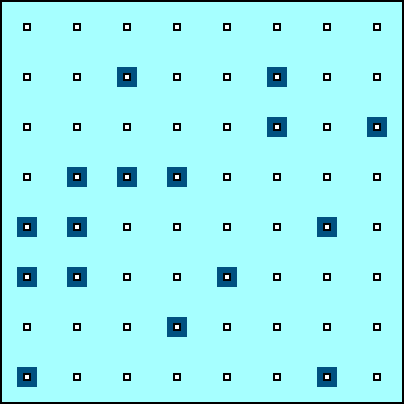
\includegraphics[width=0.22\textwidth]{Images/Sampling_SRS.png}\qquad
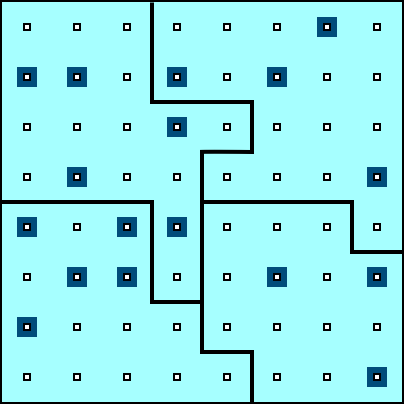
\includegraphics[width=0.22\textwidth]{Images/Sampling_StS.png}\qquad
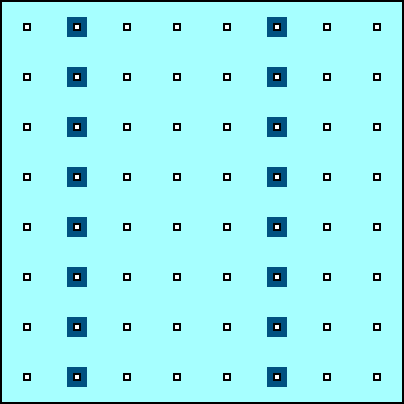
\includegraphics[width=0.22\textwidth]{Images/Sampling_SyS.png}
\\ \ \\
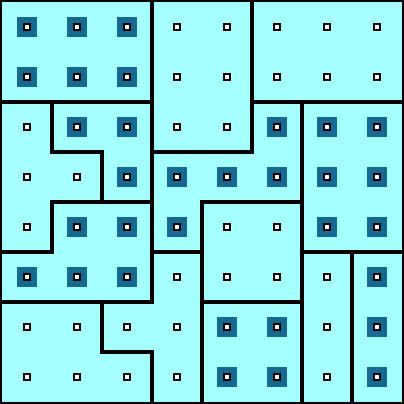
\includegraphics[width=0.22\textwidth]{Images/Sampling_ClS.png}\qquad
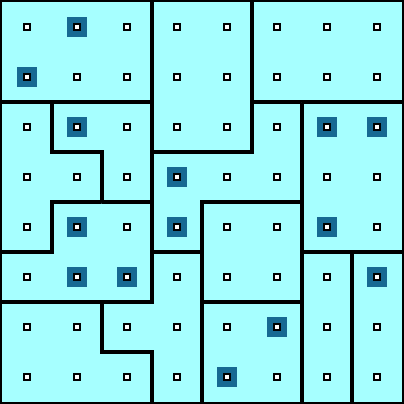
\includegraphics[width=0.22\textwidth]{Images/Sampling_MSS.png}\qquad
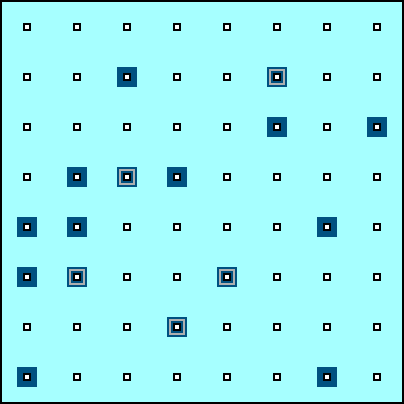
\includegraphics[width=0.22\textwidth]{Images/Sampling_MPS.png}
\caption{\small Schémas des plans d'échantillonnage. Rangée du haut, de gauche à droite: échantillonnage aléatoire simple, échantillonnage stratifié, échantillonnage systématique; rangée du bas, de gauche à droite: échantillonnage par grappes, échantillonnage à plusieurs degrés, échantillonnage à plusieurs phases.}
\hrule\label{fig:designs}
\end{figure*}
%\afterpage{\FloatBarrier}
tandis qu'avec la \textbf{r\'epartition proportionnelle} on suppose en outre que $\sigma_j=\sigma$ pour tout $j$, de sorte \`a ce que $$w_{j,P}=\frac{n_j}{n}=\frac{N_j}{N}.$$ Il existe une multitude d'autres schémas d'allocation. tels la \textbf{r\'epartition proportionnelle \`a la racine carr\'ee} qui fixe $$w_{j,S}=\frac{N_j^{1/2}}{\sum_{\ell=1}^kN_{\ell}^{1/2}};$$ c'est une allocation utile permettant de s'assurer que les plus petites strates (comme les provinces à faible population, par exemple) se voient attribuer suffisamment d'observations pour produire des estim\'es de sous-populations robustes.
 \newl Il convient de noter que si les considérations budgétaires doivent être prises en compte dans la pratique, l'approche de r\'epartition li\'ee au co\^ut ne permet pas de fixer des limites d'erreur prescrites, ce qui pourrait s'avérer problématique. La taille de l'échantillon nécessaire pour atteindre une marge d'erreur plus petite que $B$ est\small $$n_{\textrm{st},\overline{y}}=\frac{4\sum_{j=1}^k\frac{N_j\sigma_j^2}{w_j}}{N^2B^2+4\sum_{j=1}^kN_j\sigma_j^2},\quad n_{\textrm{st},\hat{\tau}}=\frac{4N^2\sum_{j=1}^k\frac{N_j\sigma_j^2}{w_j}}{N^2B^2+4\sum_{j=1}^kN_j\sigma_j^2},$$ et $$n_{\textrm{st},\hat{p}}=\frac{4\sum_{j=1}^k\frac{N_jp_j(1-p_j)}{w_j}}{N^2B^2+4\sum_{j=1}^kN_jp_j(1-p_j)},$$ \normalsize o\`u $\sigma_j^2$ et $p_j$ ont \'et\'e estim\'e au pr\'ealable, et o\`u une r\'epartition $\{w_j\}$ \`a d\'ej\`a \'et\'e choisie. \newpage\noindent  
Dans le plan d'\textbf{\'echantillonnage systématique} ($\SyS$), $n$ unités sont choisies au hasard dans la base de sondage en sélectionnant d'abord (au hasard) une unité $y_1$ parmi les premières $k=\lfloor\frac{N}{n}\rfloor$ unit\'e de la base de sondage et en ajoutant systématiquement chaque $k^{\textrm{i\`eme}}$ unit\'e à l'échantil\-lon. Une illustration en est fournie \`a la Figure~\ref{fig:designs} (en haut, à droite). \newl $\SyS$ est généralement approprié lorsque la base de sondage est déjà \textbf{ordonn\'ee} le long de la caractéristique d'intérêt, dans lequel des cas cette approche fournit plus d'infor\-ma\-tions par coût unitaire que $\SRS_FR$. \par $\SyS$ est plus simple à mettre en œuvre que $\SRS_FR$ puisqu'une seule valeur aléatoire est requise et, tout comme $\SRS_FR$, il ne nécessite pas d'informations de trame auxiliaires. Si la base de sondage est assez grande (en supposant toujours, bien s\^ur, que cette derni\`ere soit bien tri\'ee), $\SyS$ peut produire un échantillon plus largement réparti (et donc peut-être plus représentatif) que $\SRS_FR$, ce qui peut contribuer à éliminer certaines sources de biais.\newl Par contre, $\SyS$ peut introduire un biais lorsque le modèle utilisé pour l'échantillon systématique coïncide avec un tendance dans la population. De plus, une telle approche n'utilise pas les informations auxiliaires, même si de telles informations existent. \par En outre, tout avantage de précision par rapport à $\SRS_FR$ disparaît si la base de sondage est ordonnée de manière aléatoire. Finalement, Il est gênant de constater que $\SyS$ ne permet d'obtenir que des estimateurs de la variance d'échantillonnage biais\'es.\newpage\noindent \`A toutes fins pratiques, $\SyS$ se comporte comme $\SRS_FR$ pour une population aléatoire. Dans ce cas, la formule de variance $\SRS_FR$ peut fournir une approximation décente. 
\par Si la base de sondage est \textbf{ordonnée} le long de la caractéristique d'intérêt, chaque échantillon $\SyS$ contiendra certaines des plus petites valeurs ainsi que certaines des plus grandes valeurs, ce qui ne serait pas nécessairement le cas dans un échantillon général $\SRS_FR$. Cela implique que les estimateurs $\SyS$ auront des variances plus \'elev\'ees que les estimateurs $\SRS_FR$ correspondants, de sorte que l'utilisation de la formule de variance $\SRS_FR$ produit une sous-estimation de l'erreur d'échantillonnage réelle dans ce cas. \par Dans le même ordre d'idées, une population est \textbf{périodique} si la base de sondage est \textbf{périodique} le long de la caractéristique d'intérêt; un échantillon $\SyS$ qui atteint à la fois les sommets et les creux d'une tendance cyclique rendra la méthode plus conforme à $\SRS_FR$ et permettra l'utilisation de la formule de variance $\SRS_FR$ comme approximation raison\-na\-ble. Pour éviter ce problème de sous-estimation de la variance, il faut envisager de changer plusieurs fois le point de départ aléatoire.\newl 
Si $n$ divise $N$, on peut consid\'erer $\SyS$  comme un plan $\StS_FR$ dans lequel la population est classifi\'ee en $k=N/n$ strates, et une unit\'e est choise dans chaque strate. La différence entre $\SyS$ et $\StS_FR$ dans ce contexte est que seule la première unité est choisie au hasard dans $\SyS$ -- le reste de l'\'echantillon est automatiquement sélectionné sur la base de la position du premier choix. \par On peut également considérer $\SyS$ comme un échantillonnage en grappes à une étape (voir la sous-section suivante), où une unité d'échantillonnage primaire est définie comme l'un des $k=N/n$ échantillons systématiques possibles. Un $\SRS_FR$ d'une unité peut alors être tiré de ces $k$ unités primaires. L'échantillon $\SyS$ sera alors constitué de tous les éléments de l'échantillon primaire sélectionné.
\newl Les estimateurs $\SyS$ sont calculés exactement comme les estimateurs $\SRS_FR$ correspondants ; les variances sont données par  
$$\GV(\overline{y}_{\textrm{sys}})=\frac{\sigma^2}{n}[1+(n-1)\rho],\quad  \GV(\hat{\tau}_{\textrm{sys}})=N^2\GV(\overline{y}_{\textrm{sys}}),$$ et $$\GV(\hat{p}_{\textrm{sys}})=\frac{p(1-p)}{n}[1+(n-1)\rho],$$ où $\rho$ est la \textbf{corrélation intra-groupe}, qui est en général impossible à calculer exactement. \newl Les autres plans d'échantillonnage sont généralement plus complexes (dans le sens o\`u les estimateurs et les estim\'es de la variance sont plus difficiles à obtenir), mais les idées conceptuelles qui sous-tendent ces plans d'échantillonnage sont toujours assez simples ; au besoin, on trouvera des détails approfondis  dans \cite{DC_SC}.
\newpage\noindent Le plan d'\textbf{\'echantillonnage par grappes} (``cluster sampling'', $\ClS$), par exemple, est généralement utilisé lorsque le coût de la collecte des données augmente avec la ``distance'' séparant les unit\'es. La population est séparée en grappes (``clusters''), et un \'echantillon $\SRS_FR$ de grappes est sélectionné -- toutes les unités d'une grappe sélectionnée sont retenues dans l'échantillon, comme on peut le voir sur la  Figure~\ref{fig:designs} (en bas, à gauche). À titre d'exemple, si l'on cherche \`a s\'electionner des individus dans une population o\`u la base de sondage est peut-être difficile à obtenir, il pourrait être plus facile d'obtenir une base de sondage des logements et de commencer par échantillonner les logements (qui sont les grappes dans la population), puis de sélectionner tous les individus dans les logements échantillonnés. Les enquêtes $\ClS$ sont généralement moins dispendieuses et moins longues à réaliser que les enquêtes $\SRS_FR$, et elles peuvent être utilisées pour illustrer les variations ``régionales'' dans une population, mais elles seront peu utiles si la taille des grappes est trop large, et biaisées si seulement un petit nombre de grappes sont choisies.